\documentclass[11pt]{article}

\usepackage[margin=1in]{geometry}
\usepackage{amsmath}
\usepackage{graphicx}
\usepackage{float}

\title{RL Lab 5 -- Function Approximation and Control}
\author{Fotios Kapotos}
\date{}

\begin{document}

\maketitle

\section{SARSA Agent}
\subsection{Evolution of average number of steps per episode}

\begin{figure}[h]
    \centering
    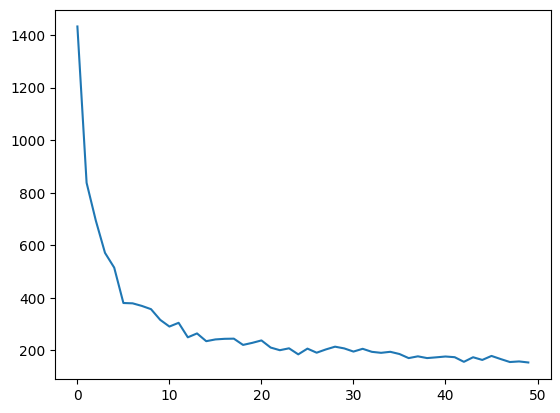
\includegraphics[width=0.48\textwidth]{figures/output_sarsa.png}
    \caption{Evolution of average number of steps per episode}
    \label{fig:cliff_results}
\end{figure}

The curve shows a clear decrease in the average number of steps per episode during the early phase of training, indicating that the agent progressively learns a more efficient policy.

\subsection{Influence of the tiles' configuration}

\begin{figure}[h]
    \centering
    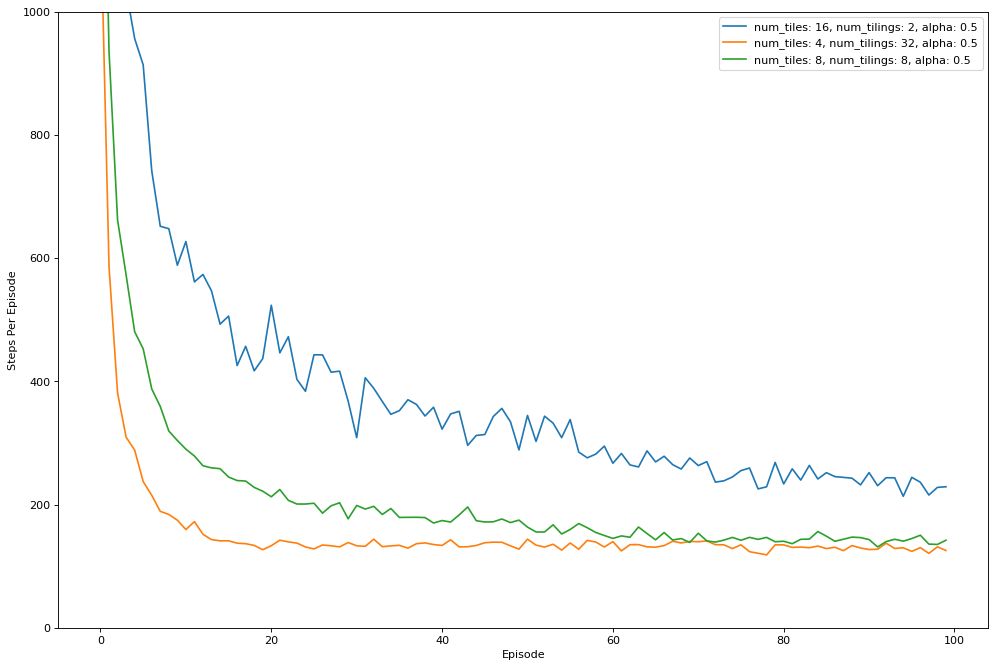
\includegraphics[width=0.48\textwidth]{figures/comp.png}
    \caption{Evolution of average number of steps per episode}
    \label{fig:cliff_results}
\end{figure}

The 8 tilings of 8x8 tiles strategy works best overall. All three configurations use the same total number of features (512), but differ in how those features are distributed. With 2 tilings of 16x16, each tiling has high resolution but the small number of tilings means limited generalization and noisier updates (larger effective step size per update). With 32 tilings of 4x4, the coarser resolution per tiling and very small effective step size (alpha/32) leads to slow convergence. The 8 tilings of 8x8 configuration strikes the best balance: enough tilings for smooth generalization across the state space, and fine enough tiles to discriminate between states.

\end{document}
